\documentclass[12pt]{article}

\setlength{\topmargin}{-.75in} \addtolength{\textheight}{2.00in}
\setlength{\oddsidemargin}{.00in} \addtolength{\textwidth}{.75in}

\usepackage{amsmath,color,graphicx,array,multirow,rotating, enumerate}
\usepackage{type1cm}
\usepackage{eso-pic}
\usepackage[hmargin=2cm,vmargin=1.3cm]{geometry}
\usepackage{mathabx}
\usepackage[rflt]{/Users/jgates/desktop/latex/floatflt}
\usepackage[table]{xcolor}
\nofiles

\def\Tab#1{\tabular[t]{>{\rule[-1ex]{0pt}{3ex}}c}#1\endtabular}
\newcolumntype{C}{@{}c@{}}

\pagestyle{empty}
\newcounter{ProbNum}
\setlength{\parindent}{0in}

% Watermark: graph paper
\newcommand\BackgroundPic{
\put(0,0){
\parbox[b][\paperheight]{\paperwidth}{%
\vfill
\centering

\includegraphics[width=\paperwidth,height=\paperheight,keepaspectratio]{/Users/jgates/desktop/latex/pics/plain.pdf}%
\vfill
}}}

%Diagram box command [v space][content]
\newcommand{\diagrambox}[2][40 mm]{
\framebox{\parbox{175 mm}{#2 \hfill \\ \vspace{#1}}}

\bigskip
}

% MakeList: [example number] [content]
\newcommand{\MakeList}[2]{
\begin{enumerate}[#1] \itemsep1pt \parskip0pt \parsep0pt  

#2
\end{enumerate}
}

\begin{document}



{\Large Problems tagged with standards:}CVPMG
\bigskip 
% Number 140
% CVPMG Units
% Draw the missing graphs
% JG

% Watermark
\AddToShipoutPicture*{\BackgroundPic}

\addtocounter {ProbNum} {1}

%\begin{floatingfigure}[r]{.3\textwidth}
%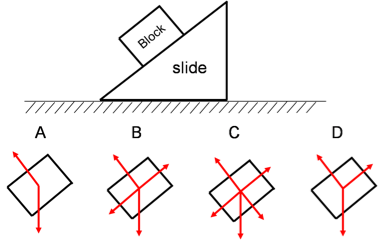
\includegraphics[scale=.4]{/Users/jgates/desktop/latex/pics/incline3.png}
%\end{floatingfigure}
 
{\bf \Large{140.}} Draw the missing graphs.

\bigskip

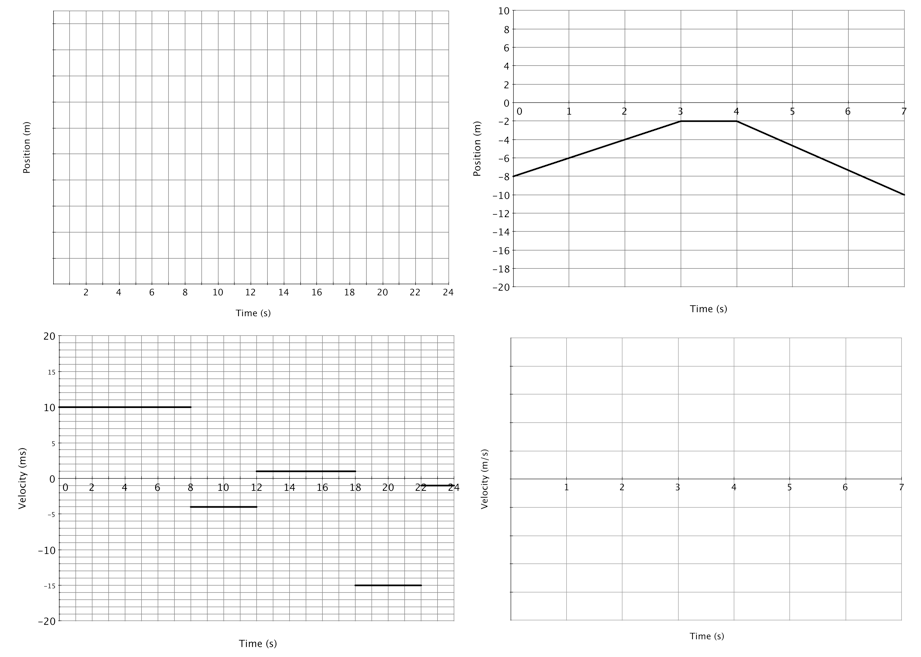
\includegraphics[scale=.57]{/Users/jgates/desktop/latex/pics/cvpmgraphs1.png}

\bigskip 
\vspace{6mm}% Number 150
% CVPMG Units
% Problem-solving, Creed and Kevin on bikes
% JG

% Watermark
\AddToShipoutPicture*{\BackgroundPic}

\addtocounter {ProbNum} {1}

%\begin{floatingfigure}[r]{.3\textwidth}
%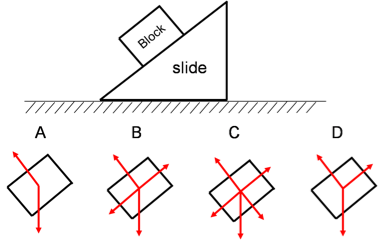
\includegraphics[scale=.4]{/Users/jgates/desktop/latex/pics/incline3.png}
%\end{floatingfigure}
 
{\bf \Large{150.}} Creed and Kevin find some bikes by the loading dock, and devise a competition: they use an 8 meter long rope to tie their bikes together and set up next to each other, facing opposite directions.  They begin next to each other, start their pedaling at the same time and ride in opposite directions, trying to see who can ride the furthest before the rope snaps tight. If Creed can pedal his bike at 4 meters per second, and he ends up 5.1 meters away from the starting point, how fast did Kevin pedal?  Solve it graphically!  Assume that they can get up to speed instantly.

%\bigskip

%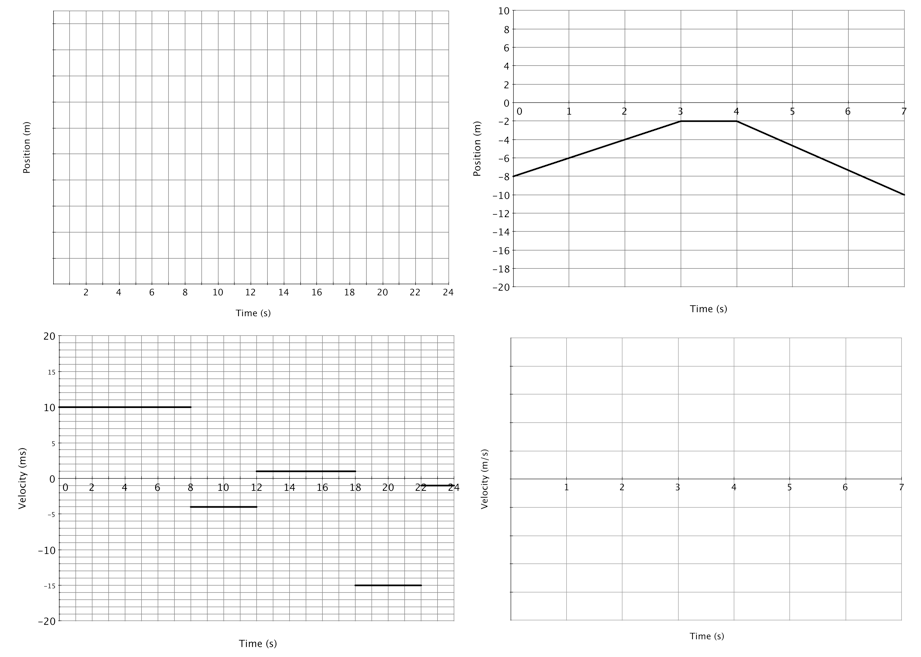
\includegraphics[scale=.57]{/Users/jgates/desktop/latex/pics/cvpmgraphs1.png}

\bigskip 
\vspace{6mm}% Number 200
% CVPMG Units
% v to x graph, quantitative
% Walker

% Watermark
\AddToShipoutPicture*{\BackgroundPic}

\addtocounter {ProbNum} {1}

%\begin{floatingfigure}[r]{.3\textwidth}
%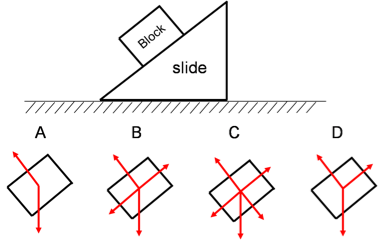
\includegraphics[scale=.4]{/Users/jgates/desktop/latex/pics/incline3.png}
%\end{floatingfigure}
 
{\bf \Large{200.}} Construct a position-vs-time graph for the motion described in the v vs t graph shown below. Assume a position of 10 meters at t = 0. Be sure to number the scale on the position axis.. 

\bigskip

%What was your original speed?  
\begin{center}
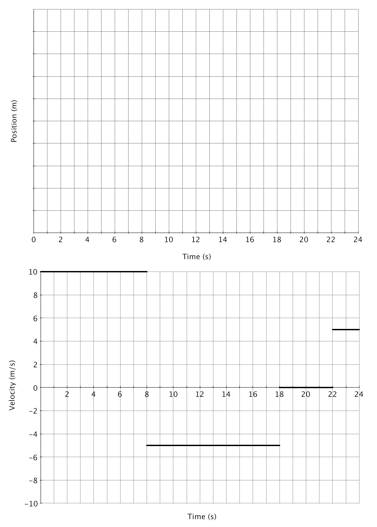
\includegraphics[scale=.77]{/Users/jgates/desktop/latex/pics/vtoxgraph1.png}
\end{center}

\bigskip 
\vspace{6mm}% Number 220
% CVPMG  Units
% Mongooses: avg v/speed, multiple representations
% JG

% Watermark
\AddToShipoutPicture*{\BackgroundPic}

\addtocounter {ProbNum} {1}

%\begin{floatingfigure}[r]{.4\textwidth}
%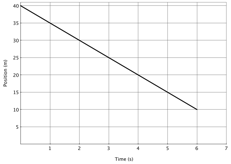
\includegraphics[scale=1]{/Users/jgates/desktop/latex/pics/flipper.png}
%\end{floatingfigure}
 
{\bf \Large{220.}} Two mongooses (mongeese?) walk around on a balance beam:

\begin{center} 
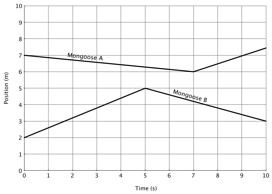
\includegraphics[scale=1]{/Users/jgates/desktop/latex/pics/mongooses.png}
\end{center}

\bigskip
Describe Mongoose A's motion in words.

\bigskip Draw a diagram describing Mongoose B's motion.

\bigskip Which mongoose has the greater average velocity?  Defend your answer.

\bigskip Which mongoose has the greater average speed?  Defend your answer.

\bigskip 
\vspace{6mm}% Number 230
% CVPMG  Units
% Dori/Danica soccer: graphical version
% JG

% Watermark
\AddToShipoutPicture*{\BackgroundPic}

\addtocounter {ProbNum} {1}

%\begin{floatingfigure}[r]{.4\textwidth}
%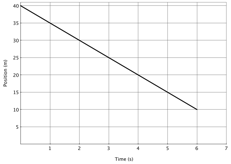
\includegraphics[scale=1]{/Users/jgates/desktop/latex/pics/flipper.png}
%\end{floatingfigure}
 
{\bf \Large{230.}} Dori's running at ${2~\tfrac{m}{s}}$ towards Tower Hill's goal line from 20 meters away when Danica lofts a ball over Dori's head.  The ball hits the ground 3 meters ahead of Dori and rolls towards the goal line at ${4~\tfrac{m}{s}}$.  

\bigskip

It takes 1.5 seconds for Dori to react to the ball; at that point, she begins running faster in order to catch up with the ball before it reaches the goal line.  
%\begin{center} 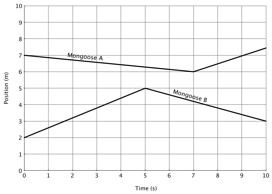
\includegraphics[scale=1]{/Users/jgates/desktop/latex/pics/mongooses.png}
%\end{center}

\bigskip

How fast does she need to run to catch up with the ball before it goes over the goal line? Use graphical problem-solving.

\bigskip 
\vspace{6mm}% Number 241
% CVPMG Units
% Football players running at each other: graphical version
% JG

% Watermark
\AddToShipoutPicture*{\BackgroundPic}

\addtocounter {ProbNum} {1}

%\begin{floatingfigure}[r]{.4\textwidth}
%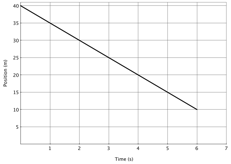
\includegraphics[scale=1]{/Users/jgates/desktop/latex/pics/flipper.png}
%\end{floatingfigure}
 
{\bf \Large{241.}} A running back carries the football down the field, running ${5.6~\tfrac{m}{s}}$.  The slower safety (running speed: ${4.5~\tfrac{m}{s}}$) runs towards him and tries to tackle him. They begin 22 meters apart and run straight at each other.  
%\begin{center} 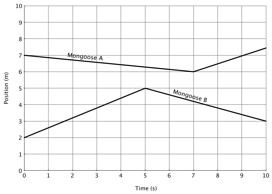
\includegraphics[scale=1]{/Users/jgates/desktop/latex/pics/mongooses.png}
%\end{center}

\bigskip

How far did the running back go before being tackled, and how much time elapsed before he was tackled? Use graphical problem solving.
 
\bigskip 
\vspace{6mm}% Number 271
% CVPMG Units
% Two objects moving, find collision time, graphical version
% JG

% Watermark
\AddToShipoutPicture*{\BackgroundPic}

\addtocounter {ProbNum} {1}

%\begin{floatingfigure}[r]{.3\textwidth}
%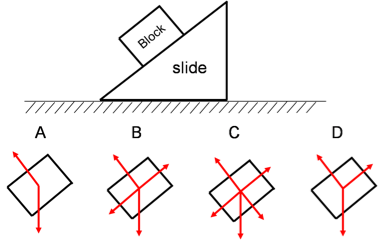
\includegraphics[scale=.4]{/Users/jgates/desktop/latex/pics/incline3.png}
%\end{floatingfigure}
 
{\bf \Large{271.}} Instead of waiting for a soccer pass to come to you, moving towards the ball can greatly increase your chances of not having the ball stolen.  A pass is made to you from 25 meters away, with a speed of ${13~\tfrac{m}{s}}$.  After a .4 second pause (your reaction time), you begin running towards the ball at ${5~\tfrac{m}{s}}$.

\bigskip
What issues might make a CVPM model of this situation less than faithful to the real situation?

\vspace{30mm}
Where (at what position) will you receive the pass? Use graphical problem-solving.

%\begin{center}
%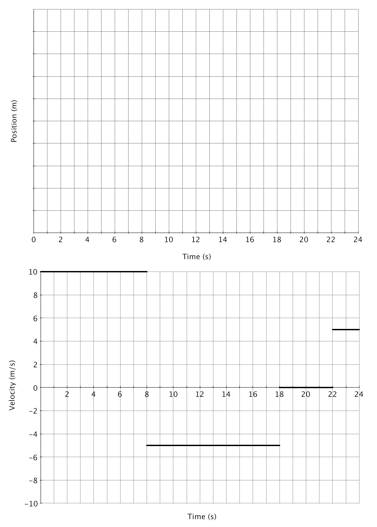
\includegraphics[scale=.77]{/Users/jgates/desktop/latex/pics/vtoxgraph1.png}
%\end{center}
 
\bigskip 
\vspace{6mm}% Number 300
% CVPMG Algebra Units
% Avg. v, speed, displacement, graph conversion
% JG

% Watermark
\AddToShipoutPicture*{\BackgroundPic}

\addtocounter {ProbNum} {1}

%\begin{floatingfigure}[r]{.3\textwidth}
%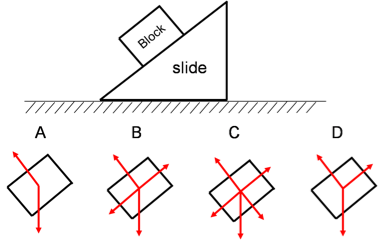
\includegraphics[scale=.4]{/Users/jgates/desktop/latex/pics/incline3.png}
%\end{floatingfigure}
 
{\bf \Large{300.}}Draw the corresponding motion graphs.

\begin{center}
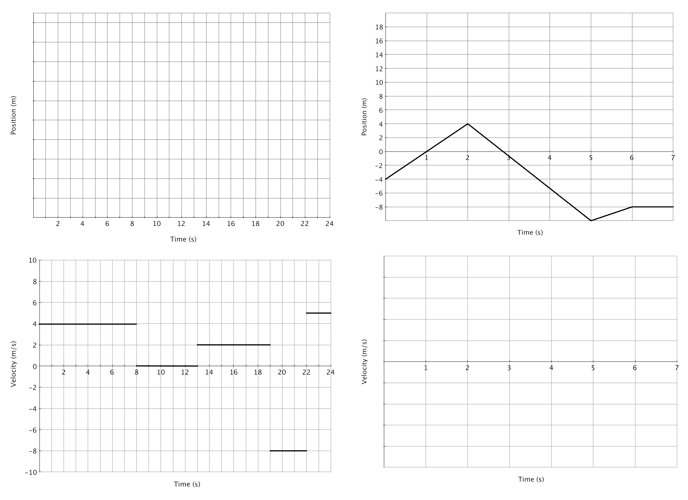
\includegraphics[scale=.77]{/Users/jgates/desktop/latex/pics/cvpmgraphs2.png}
\end{center}

\bigskip
Which motion has the greater (magnitude of) displacement?
 
\bigskip Which motion has the greater (magnitude of) average velocity?

\bigskip Which motion has the greater average speed?

\bigskip Which motion has the greater distance traveled?

\bigskip 
\vspace{6mm}% Number 310
% CVPMG  Units
% Graph description, problem-solving
% JG

% Watermark
\AddToShipoutPicture*{\BackgroundPic}

\addtocounter {ProbNum} {1}

%\begin{floatingfigure}[r]{.3\textwidth}
%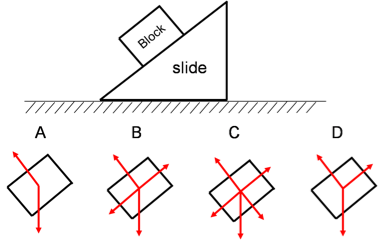
\includegraphics[scale=.4]{/Users/jgates/desktop/latex/pics/incline3.png}
%\end{floatingfigure}
 
{\bf \Large{310.}}An exciting chase has broken out between a toy police car and a toy speeder (running from the police because he foolishly doesn�t have any toy insurance).  
 
\begin{center}
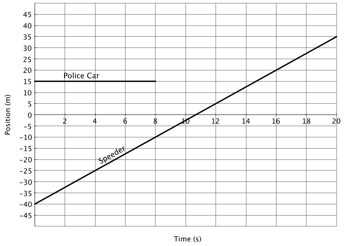
\includegraphics[scale=.87]{/Users/jgates/desktop/latex/pics/cvpm2.png}
\end{center}

\bigskip
Describe the segment of the chase shown so far, as accurately as you can (ie: including exact values).
 
\bigskip Assuming that the toy police car can get up to speed very quickly, how fast will it need to go in order to catch the speeder before ${t=~}$20 s?

\bigskip 
\vspace{6mm}% Number 320
% CVPMG Units
% Chase after distance pause: problem-solving
% JG

% Watermark
\AddToShipoutPicture*{\BackgroundPic}

\addtocounter {ProbNum} {1}

%\begin{floatingfigure}[r]{.3\textwidth}
%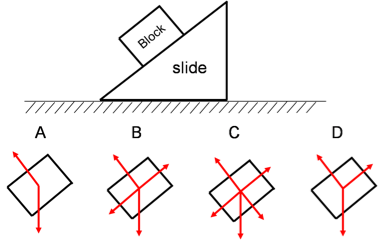
\includegraphics[scale=.4]{/Users/jgates/desktop/latex/pics/incline3.png}
%\end{floatingfigure}
 
{\bf \Large{320.}}A real police car chases down a stolen sturgeon truck.  The police car is sitting by the side of the road when the truck flies by at ${35~\tfrac{m}{s}}$.  Assume that the police officer reacts after the truck is 150 meters past her and gets up to speed instantly.  
 
%\begin{center}
%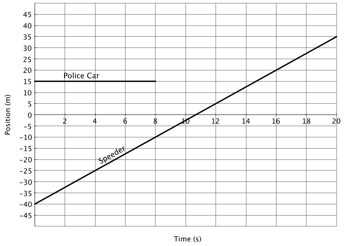
\includegraphics[scale=.87]{/Users/jgates/desktop/latex/pics/cvpm2.png}
%\end{center}

\bigskip
How fast does she need to go in order to catch the truck within 2 minutes? Use graphical problem-solving.
 
\bigskip 
\vspace{6mm}% Number 326
% CVPMG Units
% Chase after time pause: problem-solving, assumption
% JG

% Watermark
\AddToShipoutPicture*{\BackgroundPic}

\addtocounter {ProbNum} {1}

%\begin{floatingfigure}[r]{.3\textwidth}
%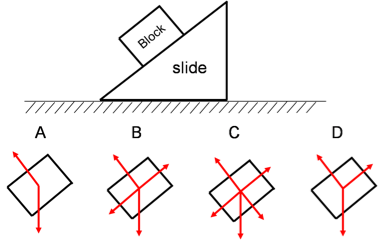
\includegraphics[scale=.4]{/Users/jgates/desktop/latex/pics/incline3.png}
%\end{floatingfigure}
 
{\bf \Large{326.}}A real police car chases down a stolen sturgeon truck.  The police car is sitting by the side of the road when the truck flies by at ${35~\tfrac{m}{s}}$.  The police officer takes 1.5 seconds to react, but we'll assume that she can get the car up to speed instantly.

%\begin{center}
%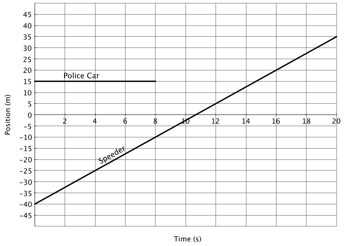
\includegraphics[scale=.87]{/Users/jgates/desktop/latex/pics/cvpm2.png}
%\end{center}

\bigskip
How fast will she have to go in order to catch the speeder within 2 km? Use graphical problem-solving.
 
\bigskip Graph (with a dotted line for the police car, but on the same axes as before) a more realistic scenario, where she requires time to get up to full speed.

\bigskip

What will this do to the top speed that will be required to catch the truck within 2 km?  Make sure that your graph agrees with this!
\bigskip \vspace{6mm}\end{document}